\documentclass[10pt]{article}
\usepackage[a4paper,margin=1.5cm,top=1.2cm,bottom=1.4cm]{geometry}
\usepackage[T1]{fontenc}
\usepackage{mathptmx}
\usepackage{microtype}
\usepackage{graphicx}
\usepackage{booktabs}
\usepackage{tabularx}
\usepackage{array}
\usepackage{xcolor}
\usepackage{placeins}
\usepackage[font=footnotesize,labelfont=bf,skip=2pt]{caption}
\usepackage{enumitem}
\usepackage{titlesec}
\usepackage[hidelinks]{hyperref}
\titlespacing*{\section}{0pt}{5pt plus 1pt}{2pt}
\titleformat{\section}{\normalsize\bfseries}{\thesection}{0.5em}{}
\titlespacing*{\subsection}{0pt}{3pt}{1pt}
\titleformat{\subsection}{\small\bfseries}{\thesubsection}{0.5em}{}
\setlength{\parskip}{2pt}
\setlength{\parindent}{0pt}
\setlist{nosep,leftmargin=1.2em}
\setlength{\textfloatsep}{5pt plus 1pt}
\setlength{\floatsep}{4pt}
\setlength{\intextsep}{4pt}
\renewcommand{\arraystretch}{1.05}
\newcolumntype{Y}{>{\raggedright\arraybackslash}X}
\pagestyle{plain}
\begin{document}
\begin{center}
{\large\bfseries Generalisation example 2: OpenML car evaluation (categorical, 4-class)}\\[2pt]
\textbf{Matric No.:} <MATRIC NO> \quad \textbf{Name:} <FULL NAME> \quad \textbf{Generalisation example} \quad \textbf{Variant-2}\\[1pt]
{\footnotesize Model: \texttt{Claude Opus 5.5 (claude-opus-5-5)} \textbar{} Interface: Agent harness - Claude Code 2.1.278 (desktop app) \textbar{} Code: \url{https://github.com/BreezyB1n/in6227-assignment1}}
\end{center}
\vspace{-4pt}
{\small \textbf{Summary.} Six ordered categorical attributes, four imbalanced classes (smallest 3.8\%), no numeric columns, no test file. Here the comparison is decisive: HGB beats LR by +0.108 macro-F1 (95\% CI +0.052 to +0.170), because the target is defined by interacting rules that an additive model cannot express.}

\section{Data exploration and cleaning}
1{,}382 training / 346 hold-out rows, no missing values or duplicates; the profiler raised only 1 flag. \begin{table}[!htb]\centering\footnotesize\setlength{\tabcolsep}{3pt}
\caption{Data issues found by the profiler and the treatment chosen (all statistics learned inside CV folds).}\label{tab:issues}
\begin{tabularx}{\linewidth}{>{\raggedright\arraybackslash}p{2.6cm} Y Y}\toprule
Issue & Evidence & Treatment and rationale\\\midrule
Severe class imbalance & {968, 307, 55, 52} training rows; ratio 18.6:1 & Primary metric macro-F1; \texttt{class\_weight} searched; stratified folds.\\
Only categorical inputs & 21 one-hot columns, all levels $\ge$ 25\% & LR: one-hot without scaling; HGB: native categorical splits; no pooling needed.\\
\bottomrule\end{tabularx}\end{table}


\section{Feature selection and engineering}
Nothing to engineer: every attribute is a design input. The levels are ordered (low $<$ med $<$ high $<$ vhigh), and a numeric encoding could help a linear model; the skill keeps them nominal because the order of \texttt{doors}=`5more' and \texttt{persons}=`more' is not numeric. This choice is worth challenging, and the next ablation to add.

\section{Model training}
LR (multinomial, one-hot) vs.\ HGB with native categorical splits; 10-fold CV because $n<2000$; macro-F1 for refit. HGB's \texttt{max\_leaf\_nodes} first landed on its upper boundary (64), so the range was widened once to 128 per the skill's rule; the re-run selected 66. Stopping: LR converged in 606 iterations; HGB early-stopped after 242 rounds. \begin{table}[!htb]\centering\footnotesize\setlength{\tabcolsep}{3pt}
\caption{Hyper-parameter search (randomised, stratified CV, refit on the primary metric) and fitted models. Gap = CV train $-$ validation primary metric (over-fitting indicator).}\label{tab:config}
\begin{tabularx}{\linewidth}{l Y Y c c c}\toprule
Model & Search & Selected & Stopping & \#inputs & Gap\\\midrule
Logistic Regression & 20 cand.\ over C [0.01, 1000] log, class\_weight $\in\{$none, balanced$\}$ & C=145, class\_weight=balanced & 606/5000 iter. & 21 & +0.034\\
Hist. Gradient Boosting & 30 cand.\ over learning\_rate [0.02, 0.3] log, max\_leaf\_nodes [8, 128], min\_samples\_leaf [2, 30], l2\_regularization [0.0001, 10] log, class\_weight $\in\{$none, balanced$\}$ & class\_weight=None, l2\_regularization=0.0144, learning\_rate=0.044, max\_leaf\_nodes=66, min\_samples\_leaf=11 & 242/2000 iter. & 6 & +0.014\\
\bottomrule\end{tabularx}\end{table}


\section{Evaluation and comparison}
\begin{table}[!htb]\centering\footnotesize\setlength{\tabcolsep}{3.2pt}
\caption{Cross-validated and held-out test performance. Class predictions are the arg-max of predicted probabilities. CIs: 1000 test-set bootstrap resamples.}\label{tab:results}
\begin{tabular}{lcccccc}\toprule
Model & CV f1\_macro (mean$\pm$sd) & Test Macro-F1 [95\% CI] & Bal.\ Acc. & Accuracy & ROC-AUC (OvR) & Log-loss\\\midrule
Prior baseline & -- & 0.206 & 0.250 & 0.699 & 0.500 & 0.838\\
Logistic Regression & 0.896$\pm$0.034 & 0.894 [0.830, 0.948] & 0.947 & 0.945 & 0.993 & 0.170\\
Hist. Gradient Boosting & 0.979$\pm$0.042 & 1.000 [1.000, 1.000] & 1.000 & 1.000 & 1.000 & 0.005\\
\bottomrule\end{tabular}\end{table}
 \begin{figure}[!ht]\centering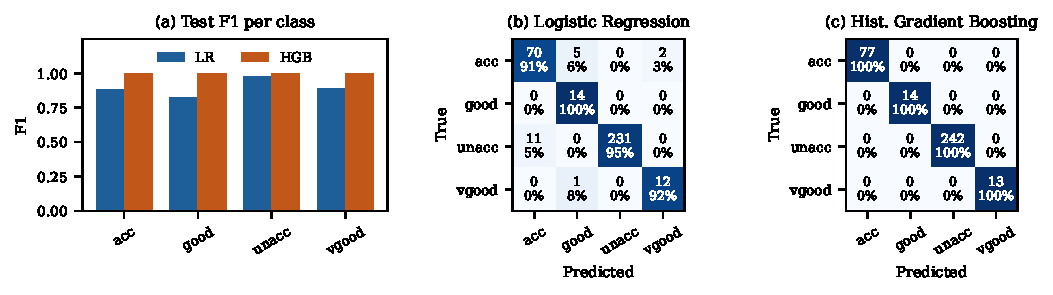
\includegraphics[width=\linewidth]{fig_results.pdf}
\caption{Hold-out set. (a) Per-class F1. (b, c) Confusion matrices (arg-max predictions).}\label{fig:results}\end{figure}
 HGB classifies the whole hold-out correctly. LR's errors concentrate where interactions matter: 11 \emph{unacc} cars predicted \emph{acc}. McNemar: 19 rows only HGB gets right, 0 the reverse ($p$ $<$0.001). Native vs.\ one-hot encoding for HGB makes no detectable difference here (Table~\ref{tab:ablation}). \begin{table}[!htb]\centering\footnotesize\setlength{\tabcolsep}{3pt}
\caption{Ablations: one decision reversed, tuned hyper-parameters kept (so $\Delta$ is conservative for the variant). $\Delta$ = change in CV f1\_macro on the same folds; sd = sd of paired fold differences ($|\Delta|<$ sd: no detectable effect); $p$: Nadeau--Bengio corrected $t$-test.}\label{tab:ablation}
\begin{tabularx}{\linewidth}{l Y r r r}\toprule
ID & Question & $\Delta$ f1\_macro & sd & $p$\\\midrule
A1\_hgb\_onehot & HGB: one-hot instead of native categorical splits & +0.0070 & 0.0284 & 0.605\\
\bottomrule\end{tabularx}\end{table}


\section{Findings and discussion}
Where the main report found a largely additive signal, this dataset is the opposite case, and the same two-model design exposes it: a perfect tree ensemble against a linear model at macro-F1 0.894. The perfect hold-out score should not be over-read: the dataset is a noise-free enumeration of a known rule hierarchy.

\FloatBarrier
\label{endofreport}

\end{document}
